% Provenance (never printed): old premiere S material on the formation of fossil
% fuels (preserved organic matter, burial, oil window, migration, trap, coal).
% Burial history of the invented Merrow Basin from figdata/grade-11/oil_window.py
% (constant geotherm, no compaction). Rifts and passive margins after the USGS
% West-Central Coastal Province fact sheet (2023-3028). Folds are defined in
% g12.02 mountain-building (Sync 0): the anticline is told in prose here, never
% defined. Sedimentary basins compared, diagenesis: Year 1/2.
\chapter{La geología del carbón, el petróleo y el gas}\label{ch:g11:fossil-fuel-geology}

Un trozo de lutita negra sacado de una antigua mina de \omterm{def:g11:fossil-fuel-geology:coal}{carbón} de
Pensilvania lleva hojas de plantas parecidas a helechos, aplastadas y
plateadas sobre la roca oscura. Crecieron en un pantano hace más de
trescientos millones de años, en el Carbonífero; enterradas antes de que
pudieran pudrirse, conservaron su forma, y el carbono de las plantas del
pantano se convirtió en \omterm{def:g11:fossil-fuel-geology:coal}{carbón}. El petróleo y el gas, que hoy se extraen
desde plataformas en alta mar, tienen el mismo tipo de origen: restos de seres
vivos que escaparon a la descomposición y que luego fueron enterrados y
calentados. Este capítulo sigue ese carbono enterrado desde el pantano y el
fondo marino hasta la capa de \omterm{def:g11:fossil-fuel-geology:coal}{carbón} y el yacimiento de petróleo.
% ledger: photo:g11-fossil-plants, ics:base.Carboniferous, ics:base.Permian, earle:coal-formation, earle:organic-preservation

\begin{omfigure}
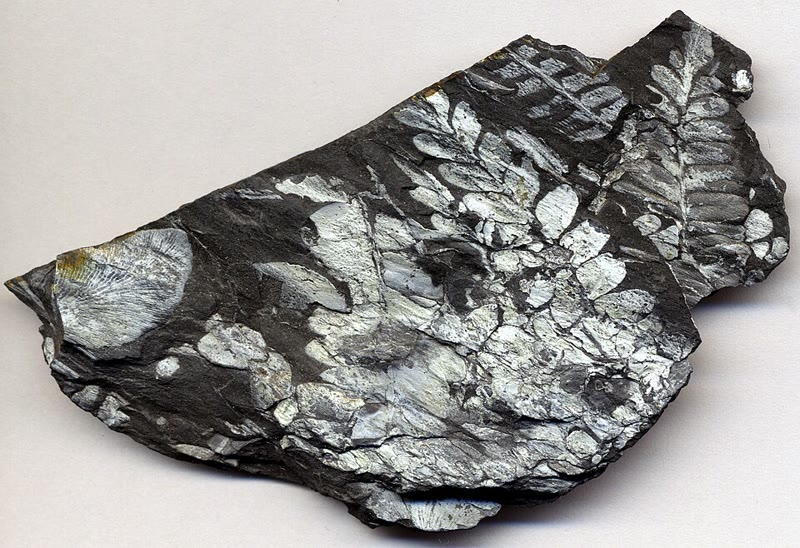
\includegraphics[height=4.4cm]{images/book2/g11-stjohn-fossil-plants.jpg}\hspace{0.03\linewidth}%
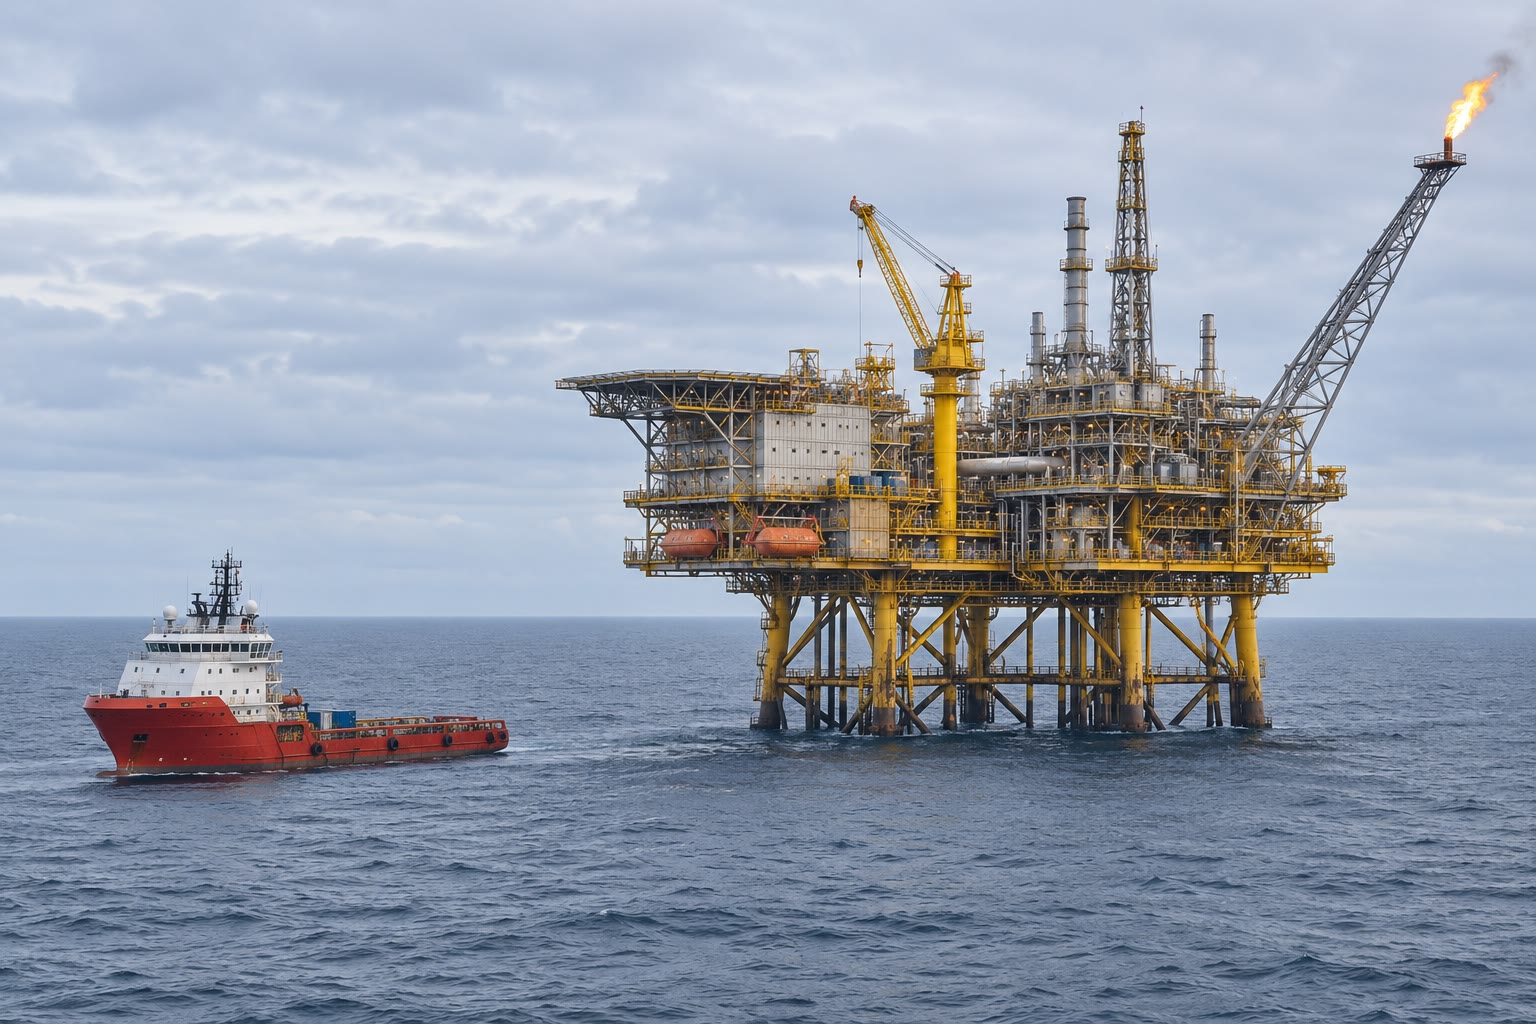
\includegraphics[height=4.4cm]{images/book2/ai/g11-offshore-platform.jpg}

{\small A la izquierda: hojas de plantas fósiles en una lutita rica en
carbono de una antigua mina de \omterm{def:g11:fossil-fuel-geology:coal}{carbón}, Pensilvania, Carbonífero; el trozo mide
unos \qty{10}{cm} de ancho. Fotografía de James St.~John (CC~BY~2.0). A la
derecha: una plataforma de producción de petróleo y gas en el mar (ilustración
generada por IA).}
\end{omfigure}
% ledger: photo:g11-fossil-plants

\begin{recall}
El \omterm{def:g11:fossil-fuel-geology:coal}{carbón}, el petróleo y el gas natural son combustibles fósiles: el petróleo
y el gas son mezclas de hidrocarburos, compuestos de carbono e hidrógeno, y al
quemar un combustible fósil se liberan energía y dióxido de carbono (los
libros de química). Las plantas y las algas fabrican materia orgánica a partir
de dióxido de carbono y agua por fotosíntesis (los libros de biología). El
\omterm{def:g11:fossil-fuel-geology:coal}{carbón}, el petróleo y el gas proceden de materia orgánica enterrada en
sedimentos, y se almacenan en rocas sedimentarias (Libro 1, año 9). Una roca
es porosa cuando contiene espacios vacíos, y permeable cuando el agua puede
fluir a través de ella (Libro 1, año 6). La temperatura sube con la
profundidad a lo largo de la \omterm{def:g11:lithosphere-asthenosphere:geotherm}{geoterma}, de 25 a \qty{30}{\degreeCelsius} por
kilómetro en los primeros kilómetros (el \cref{ch:g11:lithosphere-asthenosphere}).
\end{recall}
% ledger: usgs:gradient-29, earle:organic-preservation

\section{Conservar la materia orgánica}

La mayor parte de la materia orgánica nunca llega a ser un combustible. Una
hoja muerta o un alga muerta se la comen animales y bacterias, o reacciona con
el oxígeno del aire: en semanas o años, su carbono ha vuelto a la atmósfera en
forma de dióxido de carbono. La materia orgánica solo se conserva donde queda
aislada del oxígeno ---en el fondo de un pantano de aguas estancadas, o en un
fondo marino o lacustre cuya agua no contiene oxígeno---. Enterrada allí bajo
más sedimento, puede conservarse durante decenas o cientos de millones de años.
% ledger: earle:organic-preservation

El \omterm{def:g11:fossil-fuel-geology:coal}{carbón} procede sobre todo de plantas terrestres que se acumularon en
pantanos. El petróleo y el gas proceden sobre todo de las algas microscópicas
y del resto del plancton del mar: donde las aguas superficiales son muy
productivas, el plancton muerto cae sobre el fondo marino lo bastante deprisa
para que una parte escape a la descomposición, y queda enterrado en el fango.
% ledger: earle:coal-formation, earle:oil-window

\begin{definition}[Roca generadora; querógeno]\label{def:g11:fossil-fuel-geology:source-rock}
El \emph{querógeno}\index{querogeno@querógeno} es la materia orgánica dispersa en una
roca sedimentaria, en pequeñas partículas que no se disuelven en los
disolventes orgánicos. Una \emph{roca generadora}\index{roca generadora} es una
roca sedimentaria rica en querógeno, en la que se forman petróleo y gas cuando
se entierra y se calienta.
\end{definition}
% ledger: peters08:kerogen, earle:migration-traps

La mayoría de las \omterm{def:g11:fossil-fuel-geology:source-rock}{rocas generadoras} son lutitas y fangolitas, depositadas como
fangos ricos en materia orgánica. Cerca de la superficie, su \omterm{def:g11:fossil-fuel-geology:source-rock}{querógeno} sigue
siendo sólido: unas bacterias que viven sin oxígeno transforman parte de la
materia orgánica en metano, pero la mayor parte de ese metano vuelve a escapar
a la superficie. Para fabricar petróleo hace falta calor, y para el calor hace falta profundidad.
% ledger: earle:oil-window, peters08:kerogen

\section{Enterramiento y maduración}

\begin{definition}[Cuenca sedimentaria]\label{def:g11:fossil-fuel-geology:basin}
Una \emph{cuenca sedimentaria}\index{cuenca sedimentaria} es una región de la
corteza que se hunde durante millones de años, de modo que en ella se
acumulan sedimentos, a menudo de varios kilómetros de espesor.
\end{definition}
% ledger: usgs23:rift-salt

En una cuenca que se hunde, cada capa queda enterrada cada vez más hondo bajo
las capas que se acumulan encima. Al descender, sigue la \omterm{def:g11:lithosphere-asthenosphere:geotherm}{geoterma}: se calienta.
Su \omterm{def:g11:fossil-fuel-geology:source-rock}{querógeno} se cuece lentamente, y sus grandes moléculas se rompen en las
moléculas más pequeñas del petróleo y del gas.
% ledger: earle:oil-window

\begin{definition}[Maduración; ventana del petróleo; ventana del gas]\label{def:g11:fossil-fuel-geology:oil-window}
La \emph{maduración}\index{maduracion@maduración} de una \omterm{def:g11:fossil-fuel-geology:source-rock}{roca generadora} es la
transformación de su \omterm{def:g11:fossil-fuel-geology:source-rock}{querógeno} en petróleo y gas a medida que se entierra y se
calienta. La \emph{ventana del petróleo}\index{ventana del petroleo@ventana del petróleo} es el
intervalo de temperatura, de unos 60 a \qty{120}{\degreeCelsius}, en el que el
\omterm{def:g11:fossil-fuel-geology:source-rock}{querógeno} forma sobre todo petróleo. Por encima de unos \qty{120}{\degreeCelsius},
en la \emph{ventana del gas}\index{ventana del gas}, forma sobre todo metano.
\end{definition}
% ledger: earle:oil-window, magoon00:tps

Como la temperatura sube con la profundidad, la \omterm{def:g11:fossil-fuel-geology:oil-window}{ventana del petróleo} es
también un intervalo de profundidades. Donde la \omterm{def:g11:lithosphere-asthenosphere:geotherm}{geoterma} es una recta, es
fácil encontrarla.

\begin{proposition}[Profundidad de la ventana del petróleo]\label{prop:g11:fossil-fuel-geology:window-depth}
Sea $T_0$ la temperatura en la superficie, que sube con la profundidad $z$
según un \omterm{def:g11:lithosphere-asthenosphere:geotherm}{gradiente geotérmico} constante $G$: $T = T_0 + G z$. Entonces la
\omterm{def:g11:fossil-fuel-geology:oil-window}{ventana del petróleo} está entre las profundidades
\[
  z_{\text{techo}} = \frac{60 - T_0}{G}
  \qquad\text{y}\qquad
  z_{\text{base}} = \frac{120 - T_0}{G},
\]
con las temperaturas en \unit{\degreeCelsius}. Su espesor es $60/G$: cuanto
más pronunciada es la \omterm{def:g11:lithosphere-asthenosphere:geotherm}{geoterma}, menos profunda y más delgada es la ventana.
\end{proposition}
% ledger: earle:oil-window

\begin{proof}
El techo de la ventana es la profundidad a la que $T_0 + G z = 60$, es decir,
$z = (60 - T_0)/G$; la base, aquella a la que $T_0 + G z = 120$. La diferencia
es $(120 - 60)/G = 60/G$.
\end{proof}

Con una superficie a \qty{20}{\degreeCelsius} y un gradiente de
\qty{30}{\degreeCelsius} por kilómetro, la \omterm{def:g11:fossil-fuel-geology:oil-window}{ventana del petróleo} está entre
$40/30 \approx \qty{1.3}{km}$ y $100/30 \approx \qty{3.3}{km}$. En los sondeos
de todo Estados Unidos, el gradiente es de media de
\qty{29}{\degreeCelsius} por kilómetro, \num{25} en el este y \num{34}
en el oeste; una \omterm{def:g11:fossil-fuel-geology:source-rock}{roca generadora} suele tener que estar enterrada a más de unos
\qty{2}{km} para producir petróleo. Cuando no se dispone de ninguna medida del
\omterm{def:g11:fossil-fuel-geology:source-rock}{querógeno}, los geólogos del petróleo han considerado madura una \omterm{def:g11:fossil-fuel-geology:source-rock}{roca
generadora} enterrada bajo más de unos \qty{3}{km} de rocas más jóvenes.
% values (oil_window.py): z_top_km 1.3333, z_base_km 3.3333
% ledger: usgs:gradient-29, earle:oil-window, magoon00:tps

\begin{omfigure}
\begin{tikzpicture}
\begin{axis}[omrecord, omage, omdepth, name=burial, width=0.54\linewidth, height=5.6cm,
  xmin=0, xmax=170, ymin=0, ymax=4.5, xlabel={edad (millones de años antes de hoy)},
  ylabel={profundidad (\unit{km})}, unbounded coords=jump, clip=false,
  xtick={0,20,...,160}, ytick={0,1,...,4}]
\fill[omProp!18] (axis cs:170,1.3333) rectangle (axis cs:0,3.3333);
\fill[omThm!12] (axis cs:170,3.3333) rectangle (axis cs:0,4.5);
\node[font=\scriptsize, anchor=west, text=omProp!80!black] at (axis cs:168,1.75) {\shortstack[l]{ventana del\\petróleo}};
\node[font=\scriptsize, anchor=west, text=omThm] at (axis cs:168,3.9) {ventana del gas};
\node[font=\scriptsize, anchor=south west, text=black!60, inner sep=1pt] at (axis cs:168,1.3333) {\qty{60}{\degreeCelsius}};
\node[font=\scriptsize, anchor=south west, text=black!60, inner sep=1pt] at (axis cs:168,3.3333) {\qty{120}{\degreeCelsius}};
% computed in figdata/grade-11/oil_window.py (invented basin)
\addplot[black!45, line width=0.6pt] table[x=age, y=z150] {figdata/out/grade-11-oil_window-history.dat};
\addplot[black!45, line width=0.6pt] table[x=age, y=z120] {figdata/out/grade-11-oil_window-history.dat};
\addplot[black!45, line width=0.6pt] table[x=age, y=z95] {figdata/out/grade-11-oil_window-history.dat};
\addplot[black!45, line width=0.6pt] table[x=age, y=z66] {figdata/out/grade-11-oil_window-history.dat};
\addplot[black, line width=1.4pt] table[x=age, y=z165] {figdata/out/grade-11-oil_window-history.dat};
\draw[omDef, dashed, line width=0.8pt] (axis cs:80,0) -- (axis cs:80,4.5);
\node[font=\scriptsize, anchor=west, text=omDef, inner sep=1pt] at (axis cs:78,4.2) {se forma el anticlinal};
\fill[omThm] (axis cs:116.97,1.3333) circle (2pt);
\fill[omThm] (axis cs:51.24,3.3333) circle (2pt);
\node[font=\scriptsize, anchor=north east, inner sep=1pt] at (axis cs:100,2.3) {roca generadora};
\end{axis}
\begin{axis}[omrecord, omdepth, at={(burial.east)}, anchor=west, xshift=1.7cm, width=0.34\linewidth, height=5.6cm,
  xmin=15, xmax=50, ymin=0, ymax=7, xlabel={gradiente (\unit{\degreeCelsius/km})},
  ylabel={profundidad (\unit{km})}]
% computed in figdata/grade-11/oil_window.py (proposition, surface at 20 degC)
\addplot[name path=top, omProp, line width=1pt] table[x=G, y=z_top] {figdata/out/grade-11-oil_window-windows.dat};
\addplot[name path=base, omThm, line width=1pt] table[x=G, y=z_base] {figdata/out/grade-11-oil_window-windows.dat};
\addplot[omProp!18] fill between[of=top and base];
\node[font=\scriptsize] at (axis cs:40,1.75) {\shortstack{ventana del\\petróleo}};
\node[font=\scriptsize, anchor=south, text=omProp!80!black] at (axis cs:42,0.95) {techo};
\node[font=\scriptsize, anchor=north west, text=omThm] at (axis cs:24,4.6) {base};
\end{axis}
\end{tikzpicture}

{\small A la izquierda: historia de enterramiento de la cuenca de Merrow, una
cuenca inventada (modelo calculado, sin tener en cuenta la compactación). Cada
línea sigue una capa a lo largo del tiempo, desde el día en que se depositó en
la superficie; la línea gruesa es la \omterm{def:g11:fossil-fuel-geology:source-rock}{roca generadora}, depositada hace 165
millones de años. Con la superficie a \qty{20}{\degreeCelsius} y un gradiente
de \qty{30}{\degreeCelsius} por kilómetro, la \omterm{def:g11:fossil-fuel-geology:oil-window}{ventana del petróleo} es la banda
entre \num{1.3} y \qty{3.3}{km}. Los puntos marcan cuándo entró en ella la \omterm{def:g11:fossil-fuel-geology:source-rock}{roca
generadora} y cuándo salió hacia la \omterm{def:g11:fossil-fuel-geology:oil-window}{ventana del gas}. A la derecha: profundidad
del techo y de la base de la \omterm{def:g11:fossil-fuel-geology:oil-window}{ventana del petróleo} frente al \omterm{def:g11:lithosphere-asthenosphere:geotherm}{gradiente
geotérmico} (superficie a \qty{20}{\degreeCelsius}).}
\end{omfigure}
% values (oil_window.py): enter_oil_Ma 116.97, leave_oil_Ma 51.24, T_max 140 (20 Ma), T_today 125

Un diagrama como este es un \emph{diagrama de historia de enterramiento}: la
edad avanza de izquierda a derecha hacia la actualidad, y la profundidad, hacia
abajo. Convierte una columna de rocas, datada capa a capa, en una historia.

\begin{method}[Leer un diagrama de historia de enterramiento]\label{met:g11:fossil-fuel-geology:burial}
\begin{enumerate}
  \item Busca la línea de la \omterm{def:g11:fossil-fuel-geology:source-rock}{roca generadora}: empieza en la superficie el día
        en que se depositó la roca.
  \item Traza el techo y la base de la \omterm{def:g11:fossil-fuel-geology:oil-window}{ventana del petróleo}, como
        profundidades, a partir de la \omterm{def:g11:lithosphere-asthenosphere:geotherm}{geoterma}
        (la \cref{prop:g11:fossil-fuel-geology:window-depth}).
  \item Lee la edad a la que la línea de la \omterm{def:g11:fossil-fuel-geology:source-rock}{roca generadora} corta el techo de
        la ventana: la \omterm{def:g11:fossil-fuel-geology:source-rock}{roca generadora} empieza a producir petróleo. Lee la
        edad a la que corta la base: desde entonces produce gas.
  \item Compara esas edades con la edad de la \omterm{def:g11:fossil-fuel-geology:trap}{trampa}: solo el petróleo y el
        gas formados cuando la \omterm{def:g11:fossil-fuel-geology:trap}{trampa} ya existe pueden quedar retenidos en ella.
\end{enumerate}
\end{method}
% ledger: magoon00:tps

En la cuenca de Merrow, la \omterm{def:g11:fossil-fuel-geology:source-rock}{roca generadora} entra en la \omterm{def:g11:fossil-fuel-geology:oil-window}{ventana del petróleo}
hace unos 117 millones de años y sale de ella hace unos 51 millones de años;
su enterramiento máximo, \qty{4.0}{km} a \qty{140}{\degreeCelsius}, llega hace
20 millones de años, antes de que el levantamiento y la erosión la vuelvan a
subir. Hoy sigue en la \omterm{def:g11:fossil-fuel-geology:oil-window}{ventana del gas}. El problema de fin de semana calcula
estas edades.
% values (oil_window.py): enter_oil_Ma 116.97, leave_oil_Ma 51.24, z_max_km 4, T_max 140, T_today 125

\section{De la roca generadora a la trampa}

El petróleo y el gas son más ligeros que el agua, y los poros de las rocas
enterradas están llenos de agua. Una vez formados, salen expulsados de la \omterm{def:g11:fossil-fuel-geology:source-rock}{roca
generadora} y ascienden lentamente, a través de cualquier roca que los deje pasar.
% ledger: earle:migration-traps

\begin{definition}[Migración]\label{def:g11:fossil-fuel-geology:migration}
La \emph{migración}\index{migracion (del petroleo y del gas)@migración (del petróleo y del gas)} es el lento
desplazamiento del petróleo y del gas fuera de la \omterm{def:g11:fossil-fuel-geology:source-rock}{roca generadora} donde se
formaron, hacia arriba a través de rocas permeables, impulsado por su menor
densidad respecto del agua que los rodea.
\end{definition}
% ledger: earle:migration-traps

\begin{definition}[Roca almacén; roca sello]\label{def:g11:fossil-fuel-geology:reservoir}
Una \emph{roca almacén}\index{roca almacen@roca almacén} es una roca porosa y permeable
en la que se acumulan el petróleo y el gas: sus poros los almacenan, y las
conexiones entre ellos les permiten fluir hacia un pozo. Una \emph{roca sello}\index{roca sello} es
una roca impermeable situada sobre el almacén, que el petróleo y el gas no
pueden atravesar.
\end{definition}
% ledger: earle:migration-traps, magoon00:tps

Las areniscas y algunas calizas son buenas \omterm{def:g11:fossil-fuel-geology:reservoir}{rocas almacén}; las fangolitas, las
lutitas y la sal son buenas \omterm{def:g11:fossil-fuel-geology:reservoir}{rocas sello}. Donde nada los detiene, el petróleo
y el gas llegan a la superficie, donde rezuman y se oxidan: su carbono vuelve
a la atmósfera. Solo se acumulan donde una \omterm{def:g11:fossil-fuel-geology:reservoir}{roca sello} tiene una forma tal que
no pueden escaparse por su lado.
% ledger: earle:migration-traps, magoon00:tps

\begin{definition}[Trampa]\label{def:g11:fossil-fuel-geology:trap}
Una \emph{trampa}\index{trampa (de petroleo y gas)@trampa (de petróleo y gas)} es una disposición de \omterm{def:g11:fossil-fuel-geology:reservoir}{roca
almacén} y \omterm{def:g11:fossil-fuel-geology:reservoir}{roca sello} que retiene el petróleo y el gas, cerrándoles el camino
hacia arriba por todos los lados.
\end{definition}
% ledger: earle:migration-traps

\begin{omfigure}
\begin{tikzpicture}[font=\footnotesize, scale=0.95,
    declare function={hz(\x,\c)=\c+0.1*\x+0.7*exp(-((\x-10)^2)/2.5);}]
  \colorlet{omOil}{green!45!black}\colorlet{omGas}{red!65}
  \fill[omLithShale!70!white] (0,0) rectangle (14,-6.3);
  % overburden: limestone above a sandstone
  \fill[omLithCongl!70!white] (0,0) -- (14,0) -- plot[domain=14:0, samples=80] (\x,{-2.4+0.06*\x+0.3*exp(-((\x-10)^2)/2.5)}) -- cycle;
  \fill[omLithSand!60!white] plot[domain=0:14, samples=80] (\x,{-2.4+0.06*\x+0.3*exp(-((\x-10)^2)/2.5)}) -- plot[domain=14:0, samples=80] (\x,{hz(\x,-3.7)}) -- cycle;
  % seal (mudstone)
  \fill[omLithShale] plot[domain=0:14, samples=80] (\x,{hz(\x,-3.7)}) -- plot[domain=14:0, samples=80] (\x,{hz(\x,-4.4)}) -- cycle;
  % reservoir sandstone
  \fill[omLithSand] plot[domain=0:14, samples=80] (\x,{hz(\x,-4.4)}) -- plot[domain=14:0, samples=80] (\x,{hz(\x,-5.0)}) -- cycle;
  % oil and gas in the crest of the anticline, above the spill depth
  \begin{scope}
    \clip plot[domain=0:14, samples=80] (\x,{hz(\x,-4.4)}) -- plot[domain=14:0, samples=80] (\x,{hz(\x,-5.0)}) -- cycle;
    \fill[omOil] (8,-2.97) rectangle (13,-2.6);
    \fill[omGas] (8,-2.81) rectangle (13,-2.6);
  \end{scope}
  % source rock (black shale)
  \fill[black!70] plot[domain=0:14, samples=80] (\x,{hz(\x,-5.0)}) -- plot[domain=14:0, samples=80] (\x,{hz(\x,-5.6)}) -- cycle;
  \foreach \c in {-3.7,-4.4,-5.0,-5.6}
    \draw[black!55, line width=0.4pt] plot[domain=0:14, samples=80] (\x,{hz(\x,\c)});
  \draw[black!55, line width=0.4pt] plot[domain=0:14, samples=80] (\x,{-2.4+0.06*\x+0.3*exp(-((\x-10)^2)/2.5)});
  \draw[black!70] (0,0) -- (14,0);
  % 60 degC isotherm
  \draw[omThm, dashed, line width=0.8pt] (0,-4.3) -- (14,-4.3);
  \node[anchor=north east, text=omThm, fill=omLithShale!70!white, inner sep=1pt] at (13.95,-4.35) {\qty{60}{\degreeCelsius}};
  % migration
  \foreach \s in {0,1}
    \draw[->, omDef, line width=1.1pt] (2.7+1.2*\s,{-5.1+0.12*\s}) -- (3.2+1.2*\s,{-4.55+0.12*\s});
  \draw[->, omDef, line width=1.1pt] (4.6,-4.3) .. controls (6.5,-4.1) and (8.3,-3.7) .. (9.45,-3.0);
  % labels
  \node[anchor=west, text=white] at (0.15,-5.25) {roca generadora};
  \node[anchor=west] at (5.2,-5.75) {madura donde supera los \qty{60}{\degreeCelsius}};
  \node[anchor=west] at (0.15,-4.75) {roca almacén};
  \node[anchor=west] at (0.15,-3.97) {roca sello};
  \node[anchor=west] at (0.15,-0.4) {roca de sobrecarga};
  \node[anchor=north, text=omDef, fill=omLithShale, inner sep=1pt] at (6.2,-3.62) {migración};
  \draw[black!60] (10.0,-2.72) -- (11.4,-1.95);
  \node[anchor=south west, fill=omLithSand!60!white, inner sep=1pt] at (11.4,-1.95) {gas};
  \draw[black!60] (10.6,-2.88) -- (12.3,-2.55);
  \node[anchor=west, fill=omLithShale, inner sep=1pt] at (12.3,-2.55) {petróleo};
  \draw[black!60] (12.0,-3.45) -- (12.8,-3.15);
  \node[anchor=south, fill=omLithShale, inner sep=1pt] at (12.85,-3.15) {agua};
  \node[anchor=north] at (10,-1.0) {trampa: la bóveda de un anticlinal};
\end{tikzpicture}

{\small Un \omterm{def:g11:fossil-fuel-geology:petroleum-system}{sistema petrolífero} (un dibujo, no a escala). La \omterm{def:g11:fossil-fuel-geology:source-rock}{roca generadora},
en profundidad a la izquierda, está por debajo de la isoterma de
\qty{60}{\degreeCelsius} y produce petróleo; el petróleo y el gas salen de
ella hacia la arenisca de encima y ascienden lentamente a lo largo de ella,
bajo la \omterm{def:g11:fossil-fuel-geology:reservoir}{roca sello} de fangolita, hasta la bóveda de un anticlinal. Allí se
reúnen según su densidad: el gas arriba, el petróleo debajo y el agua más
abajo. Las \omterm{def:g11:fossil-fuel-geology:petroleum-system}{rocas de sobrecarga}, encima, entierran la \omterm{def:g11:fossil-fuel-geology:source-rock}{roca generadora} a la
profundidad suficiente para que madure.}
\end{omfigure}
% ledger: earle:migration-traps, magoon00:tps, earle:oil-window

En una \omterm{def:g11:fossil-fuel-geology:trap}{trampa}, los fluidos se ordenan según su densidad: el gas arriba, el
petróleo debajo y el agua en el fondo. La \omterm{def:g11:fossil-fuel-geology:trap}{trampa} más sencilla es un
anticlinal, una bóveda de las capas (los pliegues son el tema del \cref{ch:g12:mountain-building}). Las fallas,
los domos salinos y los cambios en las propias rocas también forman \omterm{def:g11:fossil-fuel-geology:trap}{trampas}.
% ledger: earle:migration-traps

\begin{omfigure}
\begin{tikzpicture}[font=\footnotesize, scale=0.78]
  \colorlet{omOil}{green!45!black}\colorlet{omGas}{red!65}
  % (a) anticline
  \begin{scope}
    \fill[omLithShale] (0,0) rectangle (4,3);
    \fill[omLithSand] plot[domain=0:4, samples=50] (\x,{1.0+1.0*exp(-((\x-2)^2)/1.2)}) -- plot[domain=4:0, samples=50] (\x,{1.5+1.0*exp(-((\x-2)^2)/1.2)}) -- cycle;
    \begin{scope}
      \clip plot[domain=0:4, samples=50] (\x,{1.0+1.0*exp(-((\x-2)^2)/1.2)}) -- plot[domain=4:0, samples=50] (\x,{1.5+1.0*exp(-((\x-2)^2)/1.2)}) -- cycle;
      \fill[omOil] (0,1.75) rectangle (4,3); \fill[omGas] (0,2.25) rectangle (4,3);
    \end{scope}
    \draw[black!50] (0,0) rectangle (4,3);
    \node[anchor=north, text height=1.6ex, text depth=0.3ex] at (2,-0.05) {(a) anticlinal};
  \end{scope}
  % (b) fault
  \begin{scope}[xshift=4.6cm]
    \fill[omLithShale] (0,0) rectangle (4,3);
    \begin{scope}
      \clip (0,0) -- (2.9,0) -- (2.3,3) -- (0,3) -- cycle;
      \fill[omLithSand] (0,0.6) -- (4,1.8) -- (4,2.3) -- (0,1.1) -- cycle;
      \clip (0,0.6) -- (4,1.8) -- (4,2.3) -- (0,1.1) -- cycle;
      \fill[omOil] (0,1.45) rectangle (4,3); \fill[omGas] (0,1.75) rectangle (4,3);
    \end{scope}
    \begin{scope}
      \clip (2.9,0) -- (4,0) -- (4,3) -- (2.3,3) -- cycle;
      \fill[omLithSand] (0,-0.6) -- (4,0.6) -- (4,1.1) -- (0,-0.1) -- cycle;
    \end{scope}
    \draw[black, line width=1pt] (2.9,0) -- (2.3,3);
    \draw[black!50] (0,0) rectangle (4,3);
    \node[anchor=north, text height=1.6ex, text depth=0.3ex] at (2,-0.05) {(b) falla};
  \end{scope}
  % (c) salt dome
  \begin{scope}[xshift=9.2cm]
    \fill[omLithShale] (0,0) rectangle (4,3);
    \fill[omLithSand] (0,0.9) -- (1.0,1.2) -- (1.4,1.9) -- (1.4,2.4) -- (1.0,1.7) -- (0,1.4) -- cycle;
    \fill[omLithSand] (4,0.9) -- (3.0,1.2) -- (2.6,1.9) -- (2.6,2.4) -- (3.0,1.7) -- (4,1.4) -- cycle;
    \begin{scope}
      \clip (0,0.9) -- (1.0,1.2) -- (1.4,1.9) -- (1.4,2.4) -- (1.0,1.7) -- (0,1.4) -- cycle;
      \fill[omOil] (0,1.65) rectangle (1.4,3); \fill[omGas] (0,2.05) rectangle (1.4,3);
    \end{scope}
    \begin{scope}
      \clip (4,0.9) -- (3.0,1.2) -- (2.6,1.9) -- (2.6,2.4) -- (3.0,1.7) -- (4,1.4) -- cycle;
      \fill[omOil] (2.6,1.65) rectangle (4,3); \fill[omGas] (2.6,2.05) rectangle (4,3);
    \end{scope}
    \fill[omLithEvap, draw=black!60] (1.4,0) -- (1.4,2.4) .. controls (1.4,2.85) and (2.6,2.85) .. (2.6,2.4) -- (2.6,0) -- cycle;
    \node at (2,1.0) {sal};
    \draw[black!50] (0,0) rectangle (4,3);
    \node[anchor=north, text height=1.6ex, text depth=0.3ex] at (2,-0.05) {(c) domo salino};
  \end{scope}
  % (d) stratigraphic
  \begin{scope}[xshift=13.8cm]
    \fill[omLithShale] (0,0) rectangle (4,3);
    \fill[omLithSand] (0,0.6) -- (3.5,1.95) -- (0,1.3) -- cycle;
    \begin{scope}
      \clip (0,0.6) -- (3.5,1.95) -- (0,1.3) -- cycle;
      \fill[omOil] (0,1.45) rectangle (4,3); \fill[omGas] (0,1.7) rectangle (4,3);
    \end{scope}
    \draw[black!50] (0,0) rectangle (4,3);
    \node[anchor=north, text height=1.6ex, text depth=0.3ex] at (2,-0.05) {(d) acuñamiento};
  \end{scope}
\end{tikzpicture}

{\small Cuatro tipos de \omterm{def:g11:fossil-fuel-geology:trap}{trampa} (dibujos, no a escala): arenisca almacén en
amarillo, fangolita sello en gris verdoso, petróleo en verde, gas en rojo. (a) La
bóveda de un anticlinal. (b) Un almacén inclinado cortado por una falla,
contra una fangolita al otro lado. (c) Capas dobladas hacia arriba contra un domo
salino que asciende. (d) Una arenisca que se adelgaza pendiente arriba dentro
de una fangolita, una \omterm{def:g11:fossil-fuel-geology:trap}{trampa} debida a un cambio en las propias rocas.}
\end{omfigure}
% ledger: earle:migration-traps

\begin{example}[Una trampa en un anticlinal]\label{ex:g11:fossil-fuel-geology:anticline}
Una campaña sísmica cartografía el techo de una arenisca sellada por fangolita.
Forma una bóveda cuya cresta está a \qty{1800}{m} bajo la superficie.
Alrededor de la cresta, la curva de nivel más profunda que todavía se cierra
por completo está a \qty{2050}{m}; por debajo, la arenisca se abre hacia un
lado. Un pozo en la cresta encuentra gas hasta \qty{1880}{m}. ¿Qué altura de
columna de petróleo y gas puede contener la \omterm{def:g11:fossil-fuel-geology:trap}{trampa}, y qué espesor tiene el
petróleo?

\emph{Solución.} El petróleo y el gas llenan la bóveda desde la cresta hacia
abajo; lo que baje por debajo de la última curva de nivel cerrada se derrama
hacia un lado, en el \emph{punto de derrame}, y sigue migrando. La columna
mide como mucho $2050 - 1800 = \qty{250}{m}$. Si la \omterm{def:g11:fossil-fuel-geology:trap}{trampa} está llena, el gas
ocupa los $1880 - 1800 = \qty{80}{m}$ superiores y el petróleo los
$2050 - 1880 = \qty{170}{m}$ siguientes, con agua debajo.
\end{example}
% invented numbers; ledger: earle:migration-traps

Cada una de las piezas ---una \omterm{def:g11:fossil-fuel-geology:source-rock}{roca generadora}, un almacén, una \omterm{def:g11:fossil-fuel-geology:reservoir}{roca sello}, las
rocas de encima que entierran la \omterm{def:g11:fossil-fuel-geology:source-rock}{roca generadora}, una trampa--- es necesaria,
y tienen que llegar en el orden correcto.

\begin{definition}[Sistema petrolífero]\label{def:g11:fossil-fuel-geology:petroleum-system}
Un \emph{sistema petrolífero}\index{sistema petrolifero@sistema petrolífero} es un cuerpo de \omterm{def:g11:fossil-fuel-geology:source-rock}{roca
generadora} madura junto con todo el petróleo y el gas que proceden de él, y
los elementos y procesos que necesitan: la \omterm{def:g11:fossil-fuel-geology:source-rock}{roca generadora}, la \omterm{def:g11:fossil-fuel-geology:reservoir}{roca almacén},
la \omterm{def:g11:fossil-fuel-geology:reservoir}{roca sello} y la \emph{roca de sobrecarga}\index{roca de sobrecarga} (las
rocas de encima, que entierran la \omterm{def:g11:fossil-fuel-geology:source-rock}{roca generadora}), así como la formación de
\omterm{def:g11:fossil-fuel-geology:trap}{trampas} y la generación, la \omterm{def:g11:fossil-fuel-geology:migration}{migración} y la acumulación del petróleo y del gas.
\end{definition}
% ledger: magoon00:tps

Lo que más importa es el orden. Una \omterm{def:g11:fossil-fuel-geology:trap}{trampa} que se forma después de que haya
pasado el petróleo no retiene nada: el diagrama de historia de enterramiento
fecha la generación del petróleo, la historia de los pliegues y las fallas
fecha la \omterm{def:g11:fossil-fuel-geology:trap}{trampa}, y el \omterm{def:g11:fossil-fuel-geology:petroleum-system}{sistema petrolífero} solo funciona si la \omterm{def:g11:fossil-fuel-geology:trap}{trampa} llegó
antes. Los geólogos del petróleo llaman también \emph{momento crítico} al
momento que mejor muestra a la vez la generación, la \omterm{def:g11:fossil-fuel-geology:migration}{migración} y la acumulación.
% ledger: magoon00:tps

\section{Dónde se acumulan el petróleo y el gas}

¿Dónde se reúne un \omterm{def:g11:fossil-fuel-geology:petroleum-system}{sistema petrolífero}? Necesita una cuenca que se hunda
durante mucho tiempo, aguas pobres en oxígeno para conservar la materia
orgánica, y \omterm{def:g11:fossil-fuel-geology:reservoir}{rocas sello}. Los rifts y los márgenes continentales en los que se
convierten tienen las tres cosas.
% ledger: usgs23:rift-salt

Cuando un continente empieza a partirse, como le ocurre hoy a África a lo
largo del rift de África Oriental (Libro 1, año 7), su corteza se estira y se
rompe en bloques a lo largo de \omterm{def:g11:ocean-ridges:normal-fault}{fallas normales} (el \cref{ch:g11:ocean-ridges}).
Algunos bloques se hunden, otros se inclinan, y las depresiones entre ellos se
llenan de sedimentos, a menudo de varios kilómetros de espesor, y de lagos,
cuyos fangos ricos en materia orgánica pueden convertirse en \omterm{def:g11:fossil-fuel-geology:source-rock}{rocas generadoras}. Cuando
cesa el estiramiento, la corteza adelgazada se enfría y sigue hundiéndose
lentamente, de modo que la cuenca continúa llenándose. Si después el mar
inunda una cuenca solo parcialmente conectada con el océano y se evapora,
deja capas gruesas de sal. Una vez que el rift se ha abierto en un océano,
sus bordes pasan a ser márgenes pasivos: bordes continentales situados dentro
de una placa, lejos de cualquier límite de placas, que siguen hundiéndose y
recibiendo sedimentos del continente.
% ledger: usgs23:rift-salt, usgs:pangaea-breakup

\begin{omfigure}
\begin{tikzpicture}[font=\footnotesize, x=1cm, y=0.8cm]
  \fill[omLithShale] (0,0.25) -- (1.5,0) -- (7,-0.4) -- (10,-2.2) -- (14,-2.6) -- (14,-8.0) -- (0,-8.0) -- cycle;
  % sea and land
  \fill[omSea] (1.5,0) -- (14,0) -- (14,-2.6) -- (10,-2.2) -- (7,-0.4) -- cycle;
  \draw[omRiver!60, line width=0.6pt] (1.5,0) -- (14,0);
  % marine sediments above the salt
  \fill[omLithShale] (0,0.25) -- (1.5,0) -- (7,-0.4) -- (10,-2.2) -- (14,-2.6) -- (14,-4.95) -- (11.2,-4.5) -- (11.2,-3.74) -- (0,-2.4) -- cycle;
  \fill[omLithSand] (0,-0.9) -- (6,-1.45) -- (10,-2.75) -- (14,-3.3) -- (14,-3.6) -- (10,-3.05) -- (6,-1.75) -- (0,-1.2) -- cycle;
  % salt layer and a salt dome
  \fill[omLithEvap, draw=black!50] (1.2,-2.25) -- (11.2,-3.74) -- (11.2,-4.14) -- (1.2,-2.65) -- cycle;
  \fill[omLithEvap, draw=black!50] (7.0,-3.0) .. controls (7.3,-2.6) and (7.25,-1.9) .. (7.2,-1.6)
     .. controls (7.4,-1.2) and (8.2,-1.2) .. (8.4,-1.6)
     .. controls (8.35,-2.1) and (8.3,-2.7) .. (8.7,-3.25) -- cycle;
  % continental crust with tilted blocks
  \fill[omLithGranite] (0,-2.75) -- (2.5,-3.0) -- (4.85,-4.6) -- (5.0,-3.4) -- (7.35,-5.0) -- (7.5,-3.75) -- (9.85,-5.3) -- (10.0,-4.1) -- (11.2,-5.0) -- (11.2,-6.0) -- (0,-7.6) -- cycle;
  % rift fill: lake shales (source rocks) in the half-grabens
  \fill[black!65] (2.5,-3.0) -- (4.85,-4.6) -- (5.0,-3.4) -- (4.0,-3.25) -- cycle;
  \fill[black!65] (5.0,-3.4) -- (7.35,-5.0) -- (7.5,-3.75) -- (6.5,-3.6) -- cycle;
  \fill[black!65] (7.5,-3.75) -- (9.85,-5.3) -- (10.0,-4.1) -- (9.0,-3.95) -- cycle;
  \fill[black!65] (2.5,-3.0) -- (4.0,-3.25) -- (5.0,-3.4) -- (6.5,-3.6) -- (7.5,-3.75) -- (9.0,-3.95) -- (10.0,-4.1) -- (11.2,-4.3) -- (11.2,-4.14) -- (1.2,-2.65) -- (1.2,-2.87) -- cycle;
  \draw[black!70, line width=0.8pt] (4.85,-4.6) -- (5.0,-3.4) (7.35,-5.0) -- (7.5,-3.75) (9.85,-5.3) -- (10.0,-4.1);
  % oceanic crust and mantle
  \fill[omLithBasalt] (11.2,-4.5) -- (14,-4.95) -- (14,-6.0) -- (11.2,-6.0) -- cycle;
  \fill[omLithPeridotite] (0,-7.6) -- (11.2,-6.0) -- (14,-6.0) -- (14,-8.0) -- (0,-8.0) -- cycle;
  % oil beside the salt dome
  \fill[green!45!black] (6.85,-1.5) -- (7.22,-1.65) -- (7.22,-1.95) -- (6.85,-1.75) -- cycle;
  \draw[black!60] (0,-8.0) rectangle (14,1.0);
  % labels
  \node[anchor=west] at (11.5,-1.2) {mar};
  \node[anchor=south west] at (0.1,0.3) {tierra};
  \node[anchor=west, fill=omLithShale, inner sep=1pt] at (2.2,-0.45) {sedimentos marinos};
  \node[anchor=west, fill=omLithEvap, inner sep=1pt] at (9.0,-1.25) {domo salino};
  \draw[black!60] (8.4,-1.4) -- (9.0,-1.25);
  \node[anchor=east, fill=omLithShale, inner sep=1pt] at (6.6,-2.1) {petróleo};
  \draw[black!60] (6.6,-2.1) -- (6.95,-1.75);
  \node[anchor=west, fill=omLithShale, inner sep=1pt] at (11.4,-3.35) {sal (sello)};
  \draw[black!60] (10.8,-3.7) -- (11.4,-3.35);
  \node[anchor=west, align=left] at (0.3,-4.7) {lutitas lacustres\\(rocas generadoras)};
  \draw[black!60] (2.75,-4.45) -- (4.4,-3.8);
  \node[anchor=north, align=center] at (4.0,-5.6) {corteza continental estirada:\\bloques inclinados y fallas normales};
  \node[anchor=north, align=center] at (12.6,-5.05) {corteza oceánica};
  \node[anchor=north] at (6,-7.35) {manto};
\end{tikzpicture}

{\small Un margen pasivo construido sobre un antiguo rift (un dibujo, no a
escala, con las profundidades exageradas). En el rift, bloques inclinados de
corteza continental limitados por \omterm{def:g11:ocean-ridges:normal-fault}{fallas normales} contienen lutitas
lacustres, las \omterm{def:g11:fossil-fuel-geology:source-rock}{rocas generadoras}. Una capa de sal, depositada cuando el mar
joven se evaporó, las sella; por encima se acumulan sedimentos marinos a
medida que el margen se hunde. La sal, más ligera que los sedimentos que la
rodean, asciende en domos que doblan las capas formando \omterm{def:g11:fossil-fuel-geology:trap}{trampas}.}
\end{omfigure}
% ledger: usgs23:rift-salt, earle:migration-traps

Los márgenes del Atlántico Sur se construyeron así. África y América del Sur
empezaron a separarse en el Triásico superior o el Jurásico inferior. Frente
al oeste de África Central, las depresiones del rift se llenaron con varios
kilómetros de sedimentos, entre ellos lutitas lacustres de hasta
\qty{600}{m} de espesor que contienen hasta un \qty{20}{\percent} de carbono
orgánico en masa. En el Cretácico inferior, el mar empezó a entrar, una y otra
vez, y se evaporó, dejando más de un kilómetro de sal; donde la sal ha
permanecido en su sitio, sella el petróleo y el gas de las rocas de debajo.
En el golfo de México, la sal, más ligera que los sedimentos que la rodean,
ha ascendido en domos, y las capas dobladas contra ellos son \omterm{def:g11:fossil-fuel-geology:trap}{trampas}.
% ledger: usgs23:rift-salt, earle:migration-traps

\section{El carbón}

El \omterm{def:g11:fossil-fuel-geology:coal}{carbón} se forma en tierra, sobre todo en pantanos junto a ríos y deltas,
en climas húmedos de tropicales a templados, donde las plantas crecen deprisa
y sus restos caen en aguas estancadas pobres en oxígeno. A lo largo de siglos
o milenios se acumulan como turba. Cuando un río cambia de curso, o sube el
mar, la arena y el fango entierran la turba; enterrada a más profundidad, se
comprime y se calienta.
% ledger: earle:coal-formation

\begin{definition}[Carbón; carbonificación; rango]\label{def:g11:fossil-fuel-geology:coal}
El \emph{carbón}\index{carbon@carbón} es una roca sedimentaria formada sobre todo por
restos de plantas terrestres, rica en carbono. La
\emph{carbonificación}\index{carbonificacion@carbonificación} es la transformación de la turba
en carbón, y del carbón en un carbón más rico, por enterramiento y
calentamiento. El \emph{rango}\index{rango (de un carbon)@rango (de un carbón)} de un carbón indica
hasta dónde ha llegado la carbonificación: del lignito al carbón subbituminoso
y bituminoso y a la antracita, el contenido de carbono aumenta.
\end{definition}
% ledger: earle:coal-formation, eia:coal-carbon

El lignito se forma a profundidades de unos cientos de metros a unos
\qty{1.5}{km}, hasta unos \qty{50}{\degreeCelsius}; el \omterm{def:g11:fossil-fuel-geology:coal}{carbón} bituminoso,
entre 1 y \qty{5}{km}, hasta unos \qty{150}{\degreeCelsius}; la antracita,
más allá de \qty{5}{km} y \qty{150}{\degreeCelsius}. A medida que sube el
\omterm{def:g11:fossil-fuel-geology:coal}{rango}, el carbono forma una parte cada vez mayor del \omterm{def:g11:fossil-fuel-geology:coal}{carbón}: alrededor del
25 al \qty{35}{\percent} en el lignito, y hasta del 86 al \qty{97}{\percent}
en la antracita. El metano formado por el camino queda en los poros del
\omterm{def:g11:fossil-fuel-geology:coal}{carbón}, y por eso una mina de \omterm{def:g11:fossil-fuel-geology:coal}{carbón} puede contener gas explosivo. Formar una
capa de \omterm{def:g11:fossil-fuel-geology:coal}{carbón} lleva millones de años.
% ledger: earle:coal-formation, eia:coal-carbon

\begin{omfigure}
\begin{tikzpicture}
\begin{axis}[omrecord, xbar, name=rank, width=0.5\linewidth, height=4.6cm, xmin=0, xmax=100,
  ymin=0.4, ymax=4.6, ytick={1,2,3,4},
  yticklabels={lignito, subbituminoso, bituminoso, antracita},
  xlabel={contenido de carbono (\unit{\percent})}, ymajorgrids=false]
% ledger: eia:coal-carbon
\fill[omProp!60!black!35] (axis cs:25,0.7) rectangle (axis cs:35,1.3);
\fill[omProp!70!black!55] (axis cs:35,1.7) rectangle (axis cs:45,2.3);
\fill[black!60] (axis cs:45,2.7) rectangle (axis cs:86,3.3);
\fill[black!85] (axis cs:86,3.7) rectangle (axis cs:97,4.3);
\node[font=\scriptsize, anchor=west] at (axis cs:36,1) {25--35};
\node[font=\scriptsize, anchor=west] at (axis cs:46,2) {35--45};
\node[font=\scriptsize, anchor=east, text=white] at (axis cs:85,3) {45--86};
\node[font=\scriptsize, anchor=east] at (axis cs:85,4) {86--97};
\end{axis}
\node[anchor=west] at ([xshift=0.6cm]rank.east) {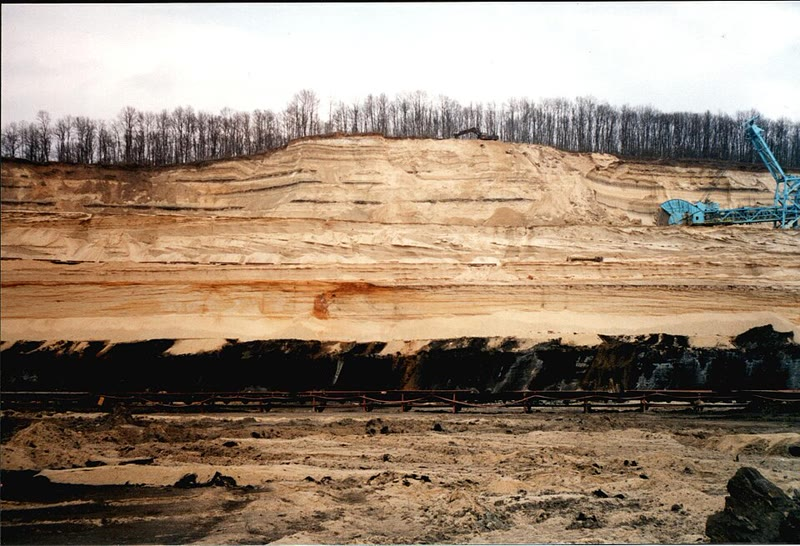
\includegraphics[height=4.0cm]{images/book2/g11-usgs-lignite-bed.jpg}};
\end{tikzpicture}

\medskip
\makebox[0.32\linewidth]{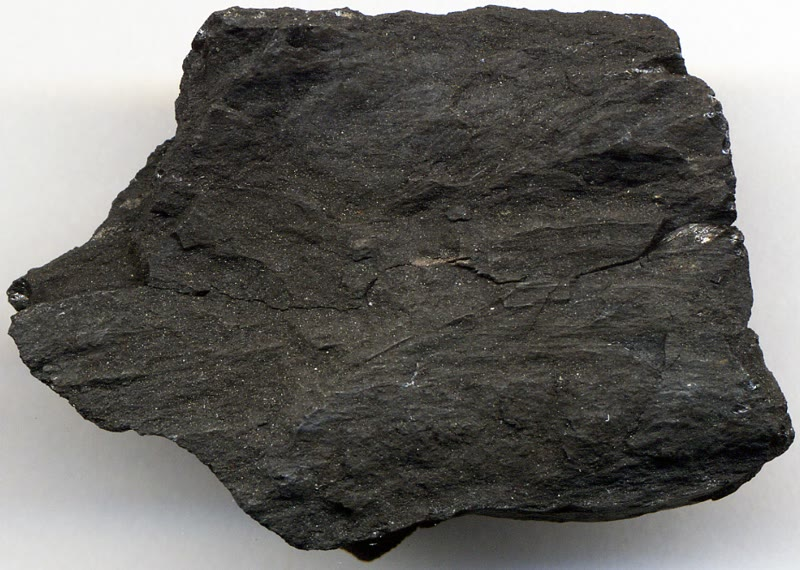
\includegraphics[height=3.2cm]{images/book2/g11-stjohn-lignite.jpg}}\hfill
\makebox[0.32\linewidth]{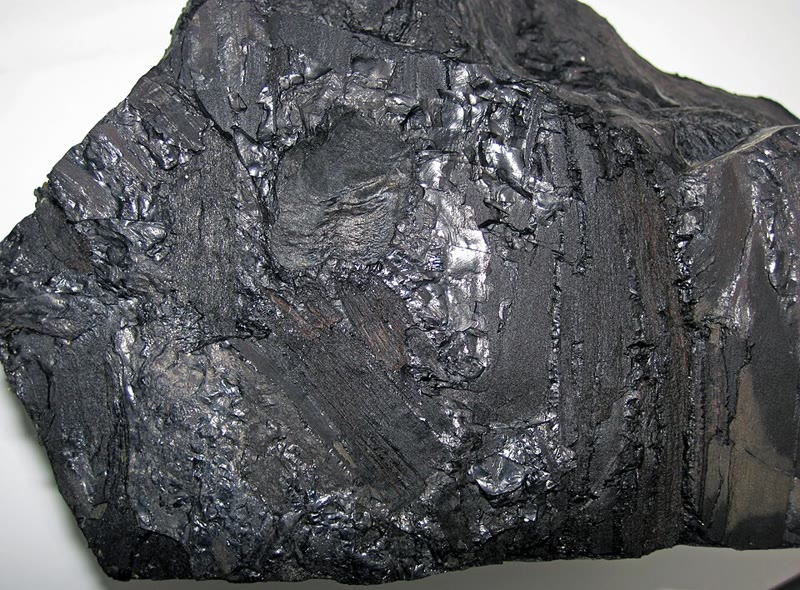
\includegraphics[height=3.2cm]{images/book2/g11-stjohn-bituminous.jpg}}\hfill
\makebox[0.32\linewidth]{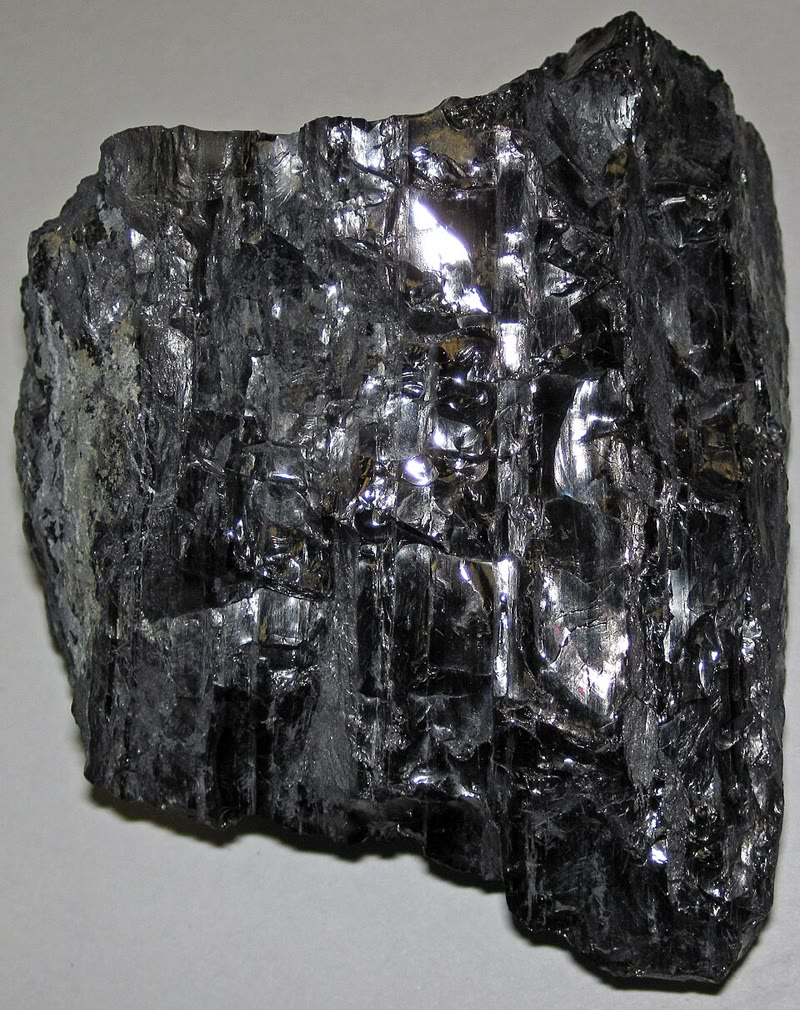
\includegraphics[height=3.2cm]{images/book2/g11-stjohn-anthracite.jpg}}

{\small Arriba a la izquierda: contenido de carbono de los \omterm{def:g11:fossil-fuel-geology:coal}{rangos} del \omterm{def:g11:fossil-fuel-geology:coal}{carbón}.
Datos: U.S. Energy Information Administration. Arriba a la derecha: un
estrato de lignito, la banda negra bajo arenas claras, al descubierto en una
mina de Rumanía; fotografía del U.S. Geological Survey (dominio público).
Abajo, desde la izquierda: lignito, de unos \qty{4.5}{cm} de ancho, de color
negro pardusco y mate; \omterm{def:g11:fossil-fuel-geology:coal}{carbón} bituminoso, con fragmentos de plantas
aplastados; antracita, negra y vítrea. Fotografías de James St.~John
(CC~BY~2.0).}
\end{omfigure}
% ledger: eia:coal-carbon, photo:g11-lignite-bed, photo:g11-coal-ranks

La turba pierde la mayor parte de su volumen por el camino. En una capa de
\omterm{def:g11:fossil-fuel-geology:coal}{carbón} del centro de Utah, la comparación de la turba cortada por un antiguo
canal fluvial con el \omterm{def:g11:fossil-fuel-geology:coal}{carbón} que falta a su lado da una razón de espesores de
alrededor de $11{:}1$: cada metro de ese \omterm{def:g11:fossil-fuel-geology:coal}{carbón} bituminoso fue antes unos once
metros de turba.
% ledger: ryer80:peat-coal

\section{Ejercicios}

\begin{exercise}[$\star$]\label{exo:g11:fossil-fuel-geology:1}
Ordena los pasos que llevan del plancton al petróleo de una \omterm{def:g11:fossil-fuel-geology:trap}{trampa}: la
\omterm{def:g11:fossil-fuel-geology:migration}{migración}; la \omterm{def:g11:fossil-fuel-geology:oil-window}{maduración} en la \omterm{def:g11:fossil-fuel-geology:oil-window}{ventana del petróleo}; el enterramiento bajo
sedimentos más jóvenes; el plancton muerto se deposita en un fondo marino
pobre en oxígeno; el petróleo se acumula bajo una \omterm{def:g11:fossil-fuel-geology:reservoir}{roca sello}; la materia
orgánica se convierte en \omterm{def:g11:fossil-fuel-geology:source-rock}{querógeno} en un fango.
\end{exercise}

\begin{exercise}[$\star$]\label{exo:g11:fossil-fuel-geology:2}
Para cada roca, di si es más probablemente una \omterm{def:g11:fossil-fuel-geology:source-rock}{roca generadora}, una \omterm{def:g11:fossil-fuel-geology:reservoir}{roca
almacén} o una \omterm{def:g11:fossil-fuel-geology:reservoir}{roca sello}: (1) una lutita oscura rica en materia orgánica;
(2) una arenisca bien clasificada con poros conectados; (3) una capa de sal;
(4) una fangolita sin materia orgánica; (5) una caliza llena de cavidades
abiertas.
\end{exercise}

\begin{exercise}[$\star$]\label{exo:g11:fossil-fuel-geology:3}
En una cuenca, la superficie está a \qty{10}{\degreeCelsius} y el \omterm{def:g11:lithosphere-asthenosphere:geotherm}{gradiente
geotérmico} es de \qty{25}{\degreeCelsius/km}. ¿Entre qué profundidades está la
\omterm{def:g11:fossil-fuel-geology:oil-window}{ventana del petróleo}? ¿Qué espesor tiene?
\end{exercise}

\begin{exercise}[$\star$]\label{exo:g11:fossil-fuel-geology:4}
(1) Ordena el lignito, la antracita, el \omterm{def:g11:fossil-fuel-geology:coal}{carbón} bituminoso y la turba según su
\omterm{def:g11:fossil-fuel-geology:coal}{rango} creciente. (2) ¿Cuál tiene el mayor contenido de carbono? (3) ¿Cuál se
formó a mayor profundidad y temperatura?
\end{exercise}

\begin{exercise}[$\star$]\label{exo:g11:fossil-fuel-geology:5}
(1) En una \omterm{def:g11:fossil-fuel-geology:trap}{trampa}, ¿por qué el gas está encima del petróleo, y el petróleo
encima del agua? (2) ¿Por qué la roca situada sobre un almacén tiene que ser
impermeable? Nombra dos rocas que sean buenas \omterm{def:g11:fossil-fuel-geology:reservoir}{rocas sello}.
\end{exercise}

\begin{exercise}[$\star\star$]\label{exo:g11:fossil-fuel-geology:6}
Dos cuencas tienen la misma temperatura en superficie, \qty{15}{\degreeCelsius}.
La cuenca A tiene un gradiente de \qty{20}{\degreeCelsius/km}, y la cuenca B,
de \qty{40}{\degreeCelsius/km}. (1) Calcula las profundidades del techo y de
la base de la \omterm{def:g11:fossil-fuel-geology:oil-window}{ventana del petróleo} en cada una. (2) Una \omterm{def:g11:fossil-fuel-geology:source-rock}{roca generadora} está a
\qty{2}{km} de profundidad en las dos cuencas. ¿Qué produce en cada una?
(3) ¿En qué cuenca tiene que ir más hondo un pozo para encontrar petróleo
formado en el lugar?
\end{exercise}

\begin{exercise}[$\star\star$]\label{exo:g11:fossil-fuel-geology:7}
Toma la razón de $11{:}1$ medida en el centro de Utah entre el espesor de una
turba y el del \omterm{def:g11:fossil-fuel-geology:coal}{carbón} en que se convirtió. (1) ¿Qué espesor de turba formó una
capa de \omterm{def:g11:fossil-fuel-geology:coal}{carbón} de \qty{3}{m} de espesor? (2) Supón que la turba se acumuló a
razón de \qty{1}{mm} al año. ¿Cuánto tardó en acumularse? (3) ¿Por qué el
pantano tuvo que estar hundiéndose durante todo ese tiempo?
\end{exercise}

\begin{exercise}[$\star\star$]\label{exo:g11:fossil-fuel-geology:8}
Usa el diagrama de historia de enterramiento de la cuenca de Merrow
(superficie a \qty{20}{\degreeCelsius}, gradiente de
\qty{30}{\degreeCelsius/km}). La \omterm{def:g11:fossil-fuel-geology:source-rock}{roca generadora} estaba a \qty{1.2}{km} de
profundidad hace 120 millones de años, a \qty{2.3}{km} hace 95 millones de
años y a \qty{4.0}{km} hace 20 millones de años. (1) Calcula su temperatura
en cada fecha. (2) En cada fecha, ¿era inmadura, estaba en la \omterm{def:g11:fossil-fuel-geology:oil-window}{ventana del
petróleo} o en la \omterm{def:g11:fossil-fuel-geology:oil-window}{ventana del gas}?
\end{exercise}

\begin{exercise}[$\star\star$]\label{exo:g11:fossil-fuel-geology:9}
El techo de una arenisca almacén forma una bóveda cuya cresta está a
\qty{2400}{m} de profundidad; su curva de nivel cerrada más profunda está a
\qty{2580}{m}. Un pozo en la cresta encuentra gas hasta \qty{2450}{m}, y luego
petróleo. (1) ¿Cuál es la altura máxima de la columna que puede contener la
\omterm{def:g11:fossil-fuel-geology:trap}{trampa}? (2) Si la \omterm{def:g11:fossil-fuel-geology:trap}{trampa} está llena, ¿qué espesor tiene el petróleo? (3) El
petróleo y el gas que siguen llegando cuando la \omterm{def:g11:fossil-fuel-geology:trap}{trampa} ya está llena: ¿adónde
van?
\end{exercise}

\begin{exercise}[$\star\star$]\label{exo:g11:fossil-fuel-geology:10}
Cuando no se dispone de ninguna medida del \omterm{def:g11:fossil-fuel-geology:source-rock}{querógeno}, los geólogos del
petróleo han considerado madura una \omterm{def:g11:fossil-fuel-geology:source-rock}{roca generadora} enterrada bajo más de
\qty{3}{km} de rocas. Con una superficie a \qty{20}{\degreeCelsius}: (1) ¿Qué
gradiente sitúa los \qty{3}{km} en el techo de la \omterm{def:g11:fossil-fuel-geology:oil-window}{ventana del petróleo}? ¿Y en
su base? (2) Con los gradientes de 25 a \qty{34}{\degreeCelsius/km} medidos en
los sondeos, ¿dónde caen los \qty{3}{km}? ¿Es razonable la regla?
\end{exercise}

\begin{exercise}[$\star\star$]\label{exo:g11:fossil-fuel-geology:11}
Tres muestras de \omterm{def:g11:fossil-fuel-geology:coal}{carbón} contienen un \qty{30}{\percent}, un \qty{70}{\percent}
y un \qty{92}{\percent} de carbono. (1) Da el \omterm{def:g11:fossil-fuel-geology:coal}{rango} de cada una. (2) Con las
profundidades y temperaturas que da el texto, ¿cuál estuvo enterrada a más
profundidad? (3) El lignito tiene un aspecto mate, negro pardusco; ¿qué
aspecto tiene la antracita?
\end{exercise}

\begin{exercise}[$\star\star\star$]\label{exo:g11:fossil-fuel-geology:12}
Entre hace 120 y hace 95 millones de años, se acumularon \qty{1100}{m} de fango
en la cuenca de Merrow. (1) Calcula el ritmo de enterramiento en metros por
millón de años. (2) Con un gradiente de \qty{30}{\degreeCelsius/km}, ¿cuántos
grados se calentó la \omterm{def:g11:fossil-fuel-geology:source-rock}{roca generadora} por millón de años? (3) Si este ritmo
hubiera continuado, ¿cuánto habría tardado la \omterm{def:g11:fossil-fuel-geology:source-rock}{roca generadora} en atravesar
toda la \omterm{def:g11:fossil-fuel-geology:oil-window}{ventana del petróleo}? (4) El modelo da unos 66 millones de años. ¿Por
qué más?
\end{exercise}

\begin{exercise}[$\star\star\star$]\label{exo:g11:fossil-fuel-geology:13}
En la cuenca de Merrow, la \omterm{def:g11:fossil-fuel-geology:source-rock}{roca generadora} estuvo en la \omterm{def:g11:fossil-fuel-geology:oil-window}{ventana del petróleo}
desde hace unos 117 hasta hace unos 51 millones de años, y el anticlinal que
atrapa el petróleo se formó hace 80 millones de años. (1) Supón que la \omterm{def:g11:fossil-fuel-geology:source-rock}{roca
generadora} produjo petróleo a un ritmo constante mientras estuvo en la
ventana. ¿Qué fracción de su petróleo se formó cuando la \omterm{def:g11:fossil-fuel-geology:trap}{trampa} ya existía?
(2) ¿Qué fue del resto? (3) Si el anticlinal se hubiera formado hace 40
millones de años, ¿qué podría contener?
\end{exercise}

\begin{exercise}[$\star\star\star$]\label{exo:g11:fossil-fuel-geology:14}
Toma la historia de enterramiento de la cuenca de Merrow (el \cref{exo:g11:fossil-fuel-geology:8}:
\qty{0.4}{km} hace 150 millones de años, \qty{1.2}{km} hace 120, \qty{2.3}{km}
hace 95, \qty{3.0}{km} hace 66, con una profundidad que crece de forma
constante entre esas fechas), pero en una cuenca más caliente: gradiente de
\qty{40}{\degreeCelsius/km}, superficie a \qty{20}{\degreeCelsius}.
(1) Calcula las profundidades del techo y de la base de la \omterm{def:g11:fossil-fuel-geology:oil-window}{ventana del
petróleo}. (2) Calcula las edades a las que la \omterm{def:g11:fossil-fuel-geology:source-rock}{roca generadora} entró en la
ventana y salió de ella. (3) El anticlinal sigue formándose hace 80 millones
de años. ¿Contendría petróleo? ¿Y gas?
\end{exercise}

\begin{exercise}[$\star\star\star$]\label{exo:g11:fossil-fuel-geology:15}
Una capa de antracita del Carbonífero aflora hoy en la superficie. El
Carbonífero terminó hace unos 299 millones de años. (1) Con las profundidades
que da el texto, ¿a qué profundidad mínima estuvo enterrada la capa? (2) Con
una superficie a \qty{15}{\degreeCelsius} y un gradiente de
\qty{30}{\degreeCelsius/km}, ¿qué temperatura alcanzó a esa profundidad? ¿Es
coherente con la temperatura que se da para la antracita? (3) ¿Qué les ha
ocurrido a las rocas que tenía encima? Da una cota inferior del ritmo medio,
en milímetros al año, suponiendo que todo ocurrió después del Carbonífero.
\end{exercise}

\section{Problema: ¿cuándo produjo petróleo la roca generadora?}

\begin{problem}[{Problema de fin de semana --- fechar el petróleo de una cuenca inventada}]
\label{pb:g11:fossil-fuel-geology:1}
% values (oil_window.py): enter_oil_Ma 116.97, leave_oil_Ma 51.238, T_max 140, T_today 125,
% after_trap_frac 0.43757; ledger ics:base.Jurassic, ics:base.Cretaceous, earle:*, magoon00:tps
Un pozo perforado a través de la cresta de un anticlinal de la cuenca de
Merrow, una cuenca inventada, atraviesa las capas de debajo. Datadas por sus
fósiles, registran cómo se rellenó la cuenca. Desde la más antigua:
\begin{center}
\small
\begin{tabular}{|l|l|l|}
\hline
\textbf{intervalo (millones de años)} & \textbf{espesor} & \textbf{rocas} \\
\hline
de 165 a 150 & \qty{400}{m} & lutita negra rica en materia orgánica, y luego fangolita \\
de 150 a 120 & \qty{800}{m} & arenisca porosa \\
de 120 a 95 & \qty{1100}{m} & fangolita \\
de 95 a 66 & \qty{700}{m} & creta \\
de 66 a 35 & \qty{700}{m} & arenas y arcillas \\
de 35 a 20 & \qty{300}{m} & arenas \\
de 20 a hoy & \qty{-500}{m} & levantamiento: erosión de los \qty{500}{m} superiores \\
\hline
\end{tabular}
\end{center}
La superficie está a \qty{20}{\degreeCelsius} y el \omterm{def:g11:lithosphere-asthenosphere:geotherm}{gradiente geotérmico} es de
\qty{30}{\degreeCelsius/km}, ambos supuestos constantes. Las capas conservan
su espesor una vez depositadas (se desprecia la compactación). El anticlinal
se formó hace 80 millones de años. Sigue la lutita negra de la base,
depositada hace 165 millones de años.

\medskip
\noindent\textbf{Parte I --- Las rocas.}
\begin{enumerate}
  \item ¿Qué capa es la \omterm{def:g11:fossil-fuel-geology:source-rock}{roca generadora}, cuál la \omterm{def:g11:fossil-fuel-geology:reservoir}{roca almacén} y cuál la \omterm{def:g11:fossil-fuel-geology:reservoir}{roca sello}?
  \item ¿Qué hizo que la lutita negra fuera rica en materia orgánica?
  \item El Jurásico duró desde hace unos \num{201.4} hasta hace unos \num{143.1}
        millones de años. ¿En qué periodo se depositó la \omterm{def:g11:fossil-fuel-geology:source-rock}{roca generadora}? ¿Y
        la arenisca?
  \item ¿Qué es el \omterm{def:g11:fossil-fuel-geology:source-rock}{querógeno}? ¿Por qué la lutita negra no produce petróleo en
        la superficie?
  \item ¿Qué espesor de rocas hay hoy encima de la \omterm{def:g11:fossil-fuel-geology:source-rock}{roca generadora}?
\end{enumerate}

\medskip
\noindent\textbf{Parte II --- El enterramiento a lo largo del tiempo.}
\begin{enumerate}[resume]
  \item Calcula la profundidad de la \omterm{def:g11:fossil-fuel-geology:source-rock}{roca generadora} hace 150, 120, 95, 66, 35
        y 20 millones de años, y hoy.
  \item Calcula el ritmo de enterramiento, en metros por millón de años,
        durante cada uno de los seis primeros intervalos.
  \item ¿Cuándo estuvo más profunda la \omterm{def:g11:fossil-fuel-geology:source-rock}{roca generadora}, y a qué profundidad?
  \item ¿Por qué disminuyó su profundidad en los últimos 20 millones de años?
  \item ¿A qué profundidad está hoy la base de la arenisca?
\end{enumerate}

\medskip
\noindent\textbf{Parte III --- La temperatura a lo largo del tiempo.}
\begin{enumerate}[resume]
  \item Calcula la temperatura de la \omterm{def:g11:fossil-fuel-geology:source-rock}{roca generadora} en cada fecha de la
        pregunta~6.
  \item ¿Entre qué profundidades está la \omterm{def:g11:fossil-fuel-geology:oil-window}{ventana del petróleo} en esta cuenca?
  \item ¿Entre qué dos fechas de la pregunta~6 pasó la \omterm{def:g11:fossil-fuel-geology:source-rock}{roca generadora} por los
        \qty{60}{\degreeCelsius}?
  \item Suponiendo que su profundidad creció de forma constante en ese
        intervalo, calcula la edad a la que llegó a \qty{60}{\degreeCelsius}.
  \item Del mismo modo, calcula cuándo llegó a \qty{120}{\degreeCelsius}.
\end{enumerate}

\medskip
\noindent\textbf{Parte IV --- La entrada en la ventana, y la trampa.}
\begin{enumerate}[resume]
  \item ¿Cuál es la temperatura más alta que alcanzó? ¿Qué produce hoy?
  \item ¿Qué fue del petróleo formado antes de que existiera el anticlinal?
  \item Suponiendo que el petróleo se formó a un ritmo constante mientras la
        \omterm{def:g11:fossil-fuel-geology:source-rock}{roca generadora} estuvo en la ventana, ¿qué fracción se formó cuando el
        anticlinal ya existía?
  \item ¿Qué fluidos esperaría encontrar el pozo en la cresta del anticlinal, y
        en qué orden desde arriba?
  \item Concluye: ¿cuándo entró la \omterm{def:g11:fossil-fuel-geology:source-rock}{roca generadora} en la \omterm{def:g11:fossil-fuel-geology:oil-window}{ventana del petróleo}?
\end{enumerate}
\end{problem}
